%% Triples with equal sum and equal reciprocal sum: the version formatted for Integers.
%% Format: the Integers article template (integers.sty, IntegersTemplate.tex) and its writing and
%% bibliography guidelines; see README.md in this folder for the sources and the changes made.
\documentclass[10pt]{article}
\usepackage{integers}

\usepackage{graphicx}
\usepackage{booktabs}
\usepackage{array}
\usepackage{hyperref}
\usepackage{xcolor}
\hypersetup{backref=true,
    pagebackref=true,
    hyperindex=true,
    colorlinks=true,
    breaklinks=true,
    urlcolor= red,
    linkcolor= blue,
    bookmarks=true,
    bookmarksopen=false,
    filecolor=black,
    citecolor=red,
    linkbordercolor=blue,
    pdftitle={Triples with equal sum and equal reciprocal sum},
    pdfauthor={Palaash Gang, Akshaj Agadi, Arjun Veluri, Jerry Wang, Jeremy Barreto, Aarin Chouthaiwale}
}
\AtBeginDocument{\hypersetup{pdfborder={0 0 0}}}

\graphicspath{{../../../}}% the figure is addressed relative to the repository root
\setlength{\emergencystretch}{3em}% keeps lines with long inline formulas within the margins

\newcommand{\Q}{\mathbb{Q}}
\newcommand{\R}{\mathbb{R}}
\newcommand{\Z}{\mathbb{Z}}
\newcommand{\PP}{\mathbb{P}}
\newcommand{\N}{\mathcal{N}}
\newcommand{\Ncl}{\mathcal{N}_{\mathrm{cl}}}
\newcommand{\ciso}{c_{\mathrm{iso}}}
\newcommand{\Orb}{\mathcal{O}}
\newtheorem{introthm}{Theorem}
\renewcommand{\theintrothm}{\Alph{introthm}}
\newtheorem{introprop}[introthm]{Proposition}
\newtheorem{introquestion}[introthm]{Question}

\title{Triples with Equal Sum and Equal Reciprocal Sum}

%% Six authors in two columns, so that the title, the authors and the abstract fit on the first page
\newcommand{\integersauthor}[3]{{\bfseries #1}\newline{\smallit #2}\newline{\tt #3}}
\author{%
  \begin{tabular}{@{}>{\centering\arraybackslash}p{2.4in}>{\centering\arraybackslash}p{2.4in}@{}}
  \integersauthor{Palaash Gang}{Indus International School,\newline Pune, India}{palaash.gang@indusschoolpune.com} &
  \integersauthor{Akshaj Agadi}{Texas A\&M University,\newline College Station, Texas, USA}{a0708@tamu.edu} \\ \noalign{\vspace{10pt}}
  \integersauthor{Arjun Veluri}{Indus International School,\newline Pune, India}{arjun.v@indusschoolpune.com} &
  \integersauthor{Jerry Wang}{University of California, Irvine,\newline Irvine, California, USA}{jerryiw@uci.edu} \\ \noalign{\vspace{10pt}}
  \integersauthor{Jeremy Barreto}{Lawrence High School,\newline Lawrenceville, New Jersey, USA}{jeremy.barreto@ltps.info} &
  \integersauthor{Aarin Chouthaiwale}{DriveChange Learning and Resource Centre,\newline Pune, India}{aarinchouthaiwale@gmail.com}
  \end{tabular}}

\begin{document}
\maketitle

\begin{abstract}
We study triples of positive integers $\{a,b,c\}$ that share both their sum and their reciprocal sum with another triple; every such triple has $1/a+1/b+1/c<1$. These are exactly the pairs of hyperbolic triangle orbifolds that the first two heat invariants cannot tell apart. Following Bremner, Guy, and Nowakowski, such triples are positive rational points on one curve of the cubic pencil $(x+y+z)(xy+yz+zx)=\Lambda xyz$, the universal elliptic curve with a rational point of order six, and reciprocation is translation by a point of order two. The torsion of these curves is then classical; we determine which torsion points are positive (the isosceles triples and the geometric progressions) and which torsion translations preserve positivity. We prove that the number $\N(X)$ of coincident pairs with sum at most $X$, and already the number of classes, is at least $(\tfrac{3\log2}{2\pi^2}+o(1))X\log X$, that $\N(X)\gg X(\log X)^2$, and, by Schinzel's method, that there are arbitrarily large classes. The dual pairs, which come from reciprocation, are rational points of a quartic del Pezzo surface, and by a theorem of Browning and Sofos the dual pairs and their multiples contribute $O(X(\log X)^5)$. An exact enumeration of all coincidences with sum at most $6000$ shows a local growth exponent falling from about $2$ near $500$ to $1.58$ at $6000$; the limiting exponent is open.
\end{abstract}

\section{Introduction}\label{sec:intro}

For a triple $x=(a,b,c)$ of positive integers write $e_1,e_2,e_3$ for its elementary symmetric functions, so that its sum and its reciprocal sum are
\[
  S(x)=e_1=a+b+c,\qquad R(x)=\frac{e_2}{e_3}=\frac1a+\frac1b+\frac1c .
\]
We call $x$ \emph{admissible} if $R(x)<1$; then every entry is at least $2$. This note is about the coincidences
\[
  S(x)=S(x'),\qquad R(x)=R(x'),\qquad x\ne x'\ \text{as unordered triples},
\]
and the smallest is $\{(2,8,8),(3,3,12)\}$, with $S=18$ and $R=\frac34$. Both triples of a coincidence are admissible (Lemma~\ref{lem:admissible}).

\subsection{Motivation}
A closed hyperbolic $2$-orbifold with underlying sphere and three cone points of orders $a,b,c$ exists exactly when $R<1$, and it is then the rigid triangle orbifold $\Orb(a,b,c)$ of area $2\pi(1-R)$. The constant term of its heat-trace expansion is $\chi/6+\sum_i(m_i^2-1)/(12m_i)=(S+R-2)/12$ \cite[(5.7)]{dggw2008} (see also the erratum \cite{dggw2017}), where $\chi=R-1$ is the orbifold Euler characteristic. So the first two heat invariants of $\Orb(a,b,c)$ determine, and are determined by, the pair $(S,R)$. Coincidences of $(S,R)$ are therefore exactly the pairs of non-isometric triangle orbifolds that two heat invariants do not distinguish. The spectral consequences are treated in the companion manuscript \emph{How much of a hyperbolic orbifold does heat hear?} \cite{gangetal-heat}; nothing here depends on it. This note is about the arithmetic of the coincidences themselves.

\subsection{Conventions}\label{sec:conventions}
A \emph{class} at sum $S$ is a set of at least two distinct admissible triples with sum $S$ and a common $R$, maximal with this property. A class of size $k$ contains $\binom k2$ \emph{pairs}. Let $n(S)$ be the number of unordered pairs at sum exactly $S$, and put
\begin{equation}\label{eq:counts}
  \N(X)=\sum_{S\le X}n(S),\qquad \Ncl(X)=\#\{\text{classes with }S\le X\}.
\end{equation}
A class, or a pair, is \emph{primitive} if the greatest common divisor of all entries of all its members is $1$; this is Schinzel's definition \cite[p.~587]{schinzel1996}. If a class at sum $S$ is multiplied by $k$, the result lies in a class at sum $kS$, which may contain further triples; scaled copies are counted at their own sums.

\subsection{Results}
Section~\ref{sec:curves} recalls that a class is a finite set of positive rational points on one plane cubic
\[
  C_\Lambda:\ (x+y+z)(xy+yz+zx)=\Lambda\,xyz,\qquad \Lambda=SR=\frac{e_1e_2}{e_3},
\]
the curve of Bremner, Guy, and Nowakowski \cite{bgn1993}. They studied it for integer $\Lambda$; coincidences need rational $\Lambda$ ($\Lambda=\frac{27}2$ for the smallest one), so we work with the whole pencil, which is the pencil of Beauville's table with singular fibres of types $I_6,I_3,I_2,I_1$ \cite[Th\'eor\`eme and Tableau, p.~658]{beauville1982}, the elliptic modular surface of $\Gamma_0(6)$, which is $\pm\Gamma_1(6)$ \cite[Table~2]{topyui2007}. With a point of order $6$, $C_\Lambda$ is the universal elliptic curve with a rational point of order $6$: for $c=-1/\Lambda$ the Weierstrass model $E_\Lambda$ of Proposition~\ref{prop:pencil} is isomorphic over $\Q$, by $x=\frac{c^2}4s+c$, $y=\frac{c^3}8\eta+\frac{c^2(c-1)}8s+c^2$, to the Tate normal form $y^2+(1-c)xy-(c+c^2)y=x^3-(c+c^2)x^2$, on which $(0,0)$, the image of $(0:1:0)=-(1:0:0)$, has order $6$, and every elliptic curve over $\Q$ with a rational point of order $6$ has this form for some $c\in\Q$; the rational parametrisations of the larger torsion structures are tabulated by Kubert \cite{kubert1976}, as Mazur records \cite[p.~156]{mazur1977}. Reciprocation $(a,b,c)\mapsto(1/a,1/b,1/c)$, under which Bremner, Guy, and Nowakowski note that solutions occur in pairs \cite[p.~117]{bgn1993}, is translation by a point of order $2$ (Proposition~\ref{prop:dual}). After rescaling to a common sum, every triple that is not a geometric progression thereby has a partner (Corollary~\ref{cor:dual}). Our results are as follows.

\begin{introthm}[Torsion, Theorem~\ref{thm:torsion}]\label{thm:T}
For rational $\Lambda\notin\{0,1,9\}$ the torsion subgroup of $C_\Lambda(\Q)$ is $\Z/6$, $\Z/12$, or $\Z/2\times\Z/6$; it is $\Z/2\times\Z/6$ exactly when $C_\Lambda$ has a rational point $(1:1:t)$, and $\Z/12$ exactly when it has a rational point $(1:r:r^2)$ with $r\ne0$. For $\Lambda>9$, a positive rational point is a torsion point exactly when two of its coordinates are equal or its coordinates, in some order, form a geometric progression.
\end{introthm}

The first sentence is, in elementary form, the classical description of the curves with a point of order $6$ whose torsion is larger, together with Mazur's theorem; the description of the positive torsion points for rational $\Lambda$, and that of the torsion translations that preserve positivity (Lemma~\ref{lem:postrans}), we have not found in the literature. For integer $\Lambda>9$ the only positive torsion points are the orderings of $(1:1:2)$ and $(1:2:2)$, at $\Lambda=10$.

\begin{introthm}[Lower bounds, Theorems~\ref{thm:iso} and~\ref{thm:loglog}]\label{thm:A}
As $X\to\infty$,
\begin{gather*}
  \N(X)\ \ge\ \Ncl(X)\ \ge\ \Big(\frac{3\log2}{2\pi^2}+o(1)\Big)X\log X,\\
  \N(X)\ \gg\ X(\log X)^2 .
\end{gather*}
\end{introthm}

The second bound comes from the dual family of Corollary~\ref{cor:dual}; it is proved for pairs only, since dual pairs can lie in one class (Theorem~\ref{thm:loglog}). Its proof does not optimise the constant, $\frac3{128\pi^4}\approx2.4\times10^{-4}$, which is so small that the second bound exceeds the first only when $\log X>438$. The dual family contributes at most $O(X(\log X)^5)$ (Proposition~\ref{prop:delpezzo}), probably of that order.

\begin{introthm}[Arbitrarily large classes, Theorem~\ref{thm:largefibres}]\label{thm:B}
For every $k$ there are infinitely many primitive classes of size at least $k$.
\end{introthm}

The proof of Theorem~\ref{thm:B} is Schinzel's argument for triples with equal sum and equal product \cite[p.~588]{schinzel1996}, applied to $C_{155/12}$; we claim no novelty for the method (Section~\ref{sec:fibres}).

\begin{introprop}[Upper bound, Proposition~\ref{prop:upper}]\label{prop:C}
$n(S)\ll_\varepsilon S^{2+\varepsilon}$, and hence $\N(X)\ll_\varepsilon X^{3+\varepsilon}$.
\end{introprop}

This bound is at the scale of the number of triples, about $S^2/12$ at sum $S$, so it does not show that coincidences are rare; we do not know a bound $n(S)=o(S^2)$. The pairs with sum $S$ are integer points of height at most $S$ on a threefold, a hypersurface in four coordinates, and $S^{2+\varepsilon}$ is the size one expects for such points in general; a power saving would need input special to this threefold, such as its elliptic fibration, which we do not have. Section~\ref{sec:growth} reports an exact enumeration of all admissible triples with $S\le4800$, extended to $S\le6000$, counting both pairs and classes. The local exponent $\log_2(\N(X)/\N(X/2))$ is about $2$ for $300\le X\le500$ and falls to $1.58$ at $X=6000$. The bounds above leave the exponent anywhere between $1$ and $3$, and the data cannot locate it. We record the question and explain what a positive answer would require (Section~\ref{sec:heuristic}).

\begin{introquestion}\label{q:intro}
Is $\N(X)=X^{1+o(1)}$?
\end{introquestion}

Equivalently, the number $A(y)$ of primitive pairs with sum at most $y$ is $y^{1+o(1)}$: by Lemma~\ref{lem:copies}, $A(X)\le\N(X)\le X\sum_{S_D\le X}1/S_D=X\int_{18^-}^Xy^{-1}\,dA(y)$, and partial summation turns $A(y)=y^{1+o(1)}$ into $\N(X)=X^{1+o(1)}$; Theorem~\ref{thm:A} is needed only for the lower bound $A(y)\gg y$, which the primitive isosceles pairs already give.

\subsection{Relation to the Literature}
The problem is the reciprocal-sum analogue of Guy's problem D16, triples with the same sum and the same product. Schinzel solved that problem through infinitely many positive rational points on the cubic $x_1+x_2+x_3=x_1x_2x_3=6$ \cite{schinzel1996}. Classes of every size for equal sums and equal products had been obtained earlier by Kelly \cite{kelly1989}, and Zhang and Cai extended Schinzel's theorem to $n$-tuples \cite{zhangcai2013}. Schinzel's curve is the fibre over $36$ of the invariant $(x+y+z)^3/xyz$ studied by Bremner and Guy \cite{bremnerguy1997}, just as $C_\Lambda$ is the fibre over $\Lambda$ of $e_1e_2/e_3$. On the equal-sum, equal-product curves, Sadek and El-Sissi showed that isosceles triples give points of order $6$ \cite[Proposition~2.5]{sadekelsissi2015}; and when the sum $M$ and the product $N$ are integers and $M$ is the sum of three distinct positive rationals $u_1>u_2>u_3$ with product $N$ with $u_1(u_2-u_3)^3\ne u_3(u_1-u_2)^3$, they showed that the rank is positive and that the torsion group is $\Z/3$, $\Z/6$, or $\Z/2\times\Z/6$ according to the number of isosceles triples on the curve \cite[Proposition~2.7 and Theorem~2.8]{sadekelsissi2015}; the last hypothesis is absent from the first preprint version, whose corresponding statements Moreland and Zieve showed to be false, with the counterexample $(3,10,24)$ \cite{morelandzieve2013}. Theorem~\ref{thm:T} is the analogue here; it differs in that geometric progressions are positive torsion points, of order $4$ or $12$. Moreland and Zieve gave conditions on rational $a,b,c$ under which $x+y+z=a+b+c$, $xyz=abc$ has infinitely many rational solutions, through families of elliptic curves of positive rank \cite{morelandzieve2013}, and Cha and coauthors studied, for a fixed sum, the sizes $n$ for which two different $n$-tuples of positive integers share the sum and the product \cite{cha2019}. Parametric families of two, three, and four triples with equal sum and equal product, and the elliptic curves of high rank they give, are constructed in \cite{ysv2024}. On the reciprocal side, Ulas proved that for every $n\ge4$ and every $k$ there are $k$ $n$-tuples of integers with equal sums of $i$th powers for $i=-1,1,2$ \cite[Theorem~3.1 and Corollary~3.4]{ulas2013}; that concerns longer tuples, three equations and no positivity. Our system is the case of three terms and exponents $-1$ and $1$ of equal sums of like powers with negative exponents. Chen's survey of the Prouhet--Tarry--Escott problem and its generalisations lists, for this type, the smallest solutions $\{4,10,12\}$, $\{5,6,15\}$ and $\{6,14,14\}$, $\{7,9,18\}$, found by Chen Shuwen (the pairs at $S=18$ and $S=20$ are smaller), chains of three such as $\{45,165,198\}$, $\{48,120,240\}$, $\{65,70,273\}$ (at $S=408$ not a complete class, which also contains $(51,102,255)$; Table~\ref{tab:fibres}), and a three-parameter solution of Choudhry \cite[Appendix~A.5.1]{chen2025}, \cite{choudhry2011}. We have not been able to consult Choudhry's paper, which was not accessible to us, so we cannot say whether his family is, or contains, the dual family or the isosceles family below. The dual family rests on a classical identity: for an $n$-tuple $x$ with nonzero entries, the tuple $\lambda/x$ with $\lambda=e_1e_n/e_{n-1}$ has the same sum and the same reciprocal sum, and for triples this is the reciprocal pairing that Bremner, Guy, and Nowakowski note \cite[p.~117]{bgn1993}. Partitions of an integer into distinct parts, of any number, with a prescribed sum of reciprocals are another line \cite{graham1963,vandoorn2025}, and counting representations by unit fractions with a prescribed reciprocal sum alone is a classical theme \cite{browningelsholtz2011,elsholtztao2013}; here the sum of the parts is prescribed as well. For integer $\Lambda=n$, Nguyen Xuan Tho proved, by Hilbert symbols on the curve $E_n$ of Section~\ref{sec:curves}, that no triple of positive integers has $e_1e_2/e_3=n$ when $4\mid n$ \cite[Theorem~1.1]{tho2021}; for these $n$ the curve $C_n$ has no positive points and carries no class. Earlier, by the same method, Bremner and Nguyen Xuan Tho had shown that $(w+x+y+z)(1/w+1/x+1/y+1/z)=n$ has no solution in positive rationals when $n=4m^2$ or $n=4m^2+4$ with $m\not\equiv2\pmod 4$ \cite[Theorems~8, 9, and~14]{bremnertho2018}, contrary to the expectation of Bremner, Guy, and Nowakowski that every $n\ge16$ is so represented \cite[p.~130]{bgn1993}, \cite{zhang2016}. Both papers concern which $n$ are represented, not how often. The same pencil appears in triangle geometry: MacLeod studied integer triangles whose circumradius and inradius have integer ratio $R/r=N$ \cite{macleod2005}, and under the substitution $(a,b,c)=(y+z,z+x,x+y)$ one has $R/r=2abc/((a+b-c)(b+c-a)(c+a-b))=(\Lambda-1)/4$, so such triangles are positive rational points of $C_{4N+1}$. The same curves carry a representation problem of Bremner and Macleod: under $(x,y,z)=(b+c,c+a,a+b)$, $\frac a{b+c}+\frac b{c+a}+\frac c{a+b}=N$ becomes $C_{2N+6}$, and their elliptic curve is $E_{2N+6}$ \cite{bremnermacleod2014}. For integer $N$ they determine its torsion \cite[Lemma~2.1]{bremnermacleod2014}, show that the solutions with $a,b,c>0$, which form a subregion of the positive triangle, come from the bounded real component \cite[Section~4]{bremnermacleod2014}, as in Lemma~\ref{lem:egg} here, prove that there are none for odd $N$ \cite[Theorem~5.1 and Corollary~5.2]{bremnermacleod2014}, which on that subregion is the case $4\mid\Lambda$ of the later theorem of Nguyen Xuan Tho, and show that the smallest positive solutions can be enormous (their Table~2 is corrected in \cite{bremnermacleod2025}). As far as we know, the counting function $\N(X)$, the bounds of Theorem~\ref{thm:A} and Proposition~\ref{prop:C}, and the exhaustive enumeration are new, while individual coincidences are in \cite{chen2025} and a parametric family in \cite{choudhry2011}; the geometry of Sections~\ref{sec:curves}--\ref{sec:dual} is largely in \cite{bgn1993}, \cite{beauville1982} and \cite{kubert1976}, and we credit it there.

\section{The Curves \texorpdfstring{$C_\Lambda$}{C\_Lambda}}\label{sec:curves}

\begin{lemma}[Coincidences are admissible]\label{lem:admissible}
If two distinct triples of positive integers have the same sum and the same reciprocal sum, both are admissible.
\end{lemma}

\begin{proof}
Let $x=(a,b,c)$ with $a\le b\le c$ and $R(x)\ge1$, and let $x'$ be a triple with $S(x')=S(x)$ and $R(x')=R(x)$; we show $x'=x$. If $a\ge4$ then $R\le\frac34$; if $a=3$ then $R\ge1$ forces $b=c=3$; if $a=2$ then $\frac1b+\frac1c\ge\frac12$ forces $b=2$, or $b=3$ and $c\le6$, or $b=c=4$. So the triples with $R\ge1$ are those with $a=1$ (where $R>1$), the triples $(2,2,c)$ (where $R>1$), the triples $(2,3,c)$ with $3\le c\le6$, and $(2,4,4)$ and $(3,3,3)$; among the last three kinds $R=1$ exactly for $(2,3,6)$, $(2,4,4)$, and $(3,3,3)$. As $R(x')\ge1$, the triple $x'$ is in this list. If $x$ and $x'$ have the same least entry $a$, their other two entries have the same sum $S-a$ and the same reciprocal sum $R-1/a$, hence the same product, so $x'=x$. Otherwise one of them, say $x$, has least entry $1$, or the least entries are $2$ and $3$; as $(3,3,3)$ is the only listed triple with least entry $3$, the two then have sum $9$ and one is $(3,3,3)$. In the second case the other is $(2,2,5)$ or $(2,3,4)$, with $R=\frac65$ or $\frac{13}{12}$, not $1$. In the first case $R>1$, so $x'$ is $(2,2,c')$ with $c'\ge2$ or $(2,3,c')$ with $3\le c'\le5$. If $x'=(2,2,c')$, then $b+c=c'+3$ and $(b+c)/bc=1/c'$, so $b$ and $c$ are the roots of $w^2-(c'+3)w+c'(c'+3)$, whose discriminant $3(c'+3)(1-c')$ is negative. If $x'=(2,3,c')$, then $b+c=c'+4$ and $(b+c)/bc=1/c'-\frac16$, so $bc=6c'(c'+4)/(6-c')$, and the discriminant $(c'+4)(24-22c'-c'^2)/(6-c')$ is negative.
\end{proof}

\begin{proposition}[Classes are points on a cubic]\label{prop:reformulation}
Two triples with the same sum have the same $R$ if and only if they have the same $\Lambda=e_1e_2/e_3$. Conversely, let $k\ge2$, let $x_1,\dots,x_k$ be primitive triples, no one of them proportional to a permutation of another, of positive integers with a common $\Lambda$, let $s_i$ be the sum of $x_i$, and let $L=\operatorname{lcm}(s_1,\dots,s_k)$. Then the triples $(L/s_i)x_i$ lie in one primitive class at sum $L$, which may contain further triples, and any sum at which multiples of all the $x_i$ occur is a multiple of $L$.
\end{proposition}

\begin{proof}
The first statement is immediate from $\Lambda=SR$. The rescaled triples have sum $L$ and $R=\Lambda/L$, they are distinct unordered triples by the hypothesis, and they are admissible by Lemma~\ref{lem:admissible}. If $d$ divides every entry of every $(L/s_i)x_i$ then, each $x_i$ being primitive, $d\mid L/s_i$ for all $i$, so every $s_i$ divides $L/d$; hence $L\mid L/d$ and $d=1$. An integer triple proportional to the primitive triple $x_i$ is $c\,x_i$ with $c\in\Z$, so a common sum $S$ for all of them forces $s_i\mid S$ for every $i$, that is $L\mid S$.
\end{proof}

So a class is a finite set of positive rational points on $C_\Lambda$, and scaling a class does not move its points. Bremner, Guy, and Nowakowski observed the scale invariance for integer $\Lambda$ \cite[p.~117]{bgn1993}. By the arithmetic--harmonic mean inequality $\Lambda=e_1\cdot R\ge9$ at positive points, with equality only at $(1:1:1)$.

\begin{proposition}[The pencil]\label{prop:pencil}
Since $(x+y)(y+z)(z+x)=e_1e_2-e_3$, the curve $C_\Lambda$ is the member $t=1-\Lambda$ of the pencil
\[
  (X+Y)(Y+Z)(Z+X)+t\,XYZ=0
\]
of Beauville's table with singular fibres of types $I_6,I_3,I_2,I_1$ \cite[Th\'eor\`eme and Tableau, p.~658]{beauville1982}. Its singular members are at $\Lambda=\infty,1,0,9$, with fibres of these types on the rational elliptic surface obtained by blowing up the base points (at $\Lambda=\infty$ the plane member is the triangle $xyz=0$). For every other $\Lambda$ the curve $C_\Lambda$ is smooth of genus one, and the maps
\[
  s=-\frac{4e_2}{z^2},\qquad \eta=\frac{4\Lambda(\Lambda-1)(x-y)}{x+y-(\Lambda-1)z},\qquad
  \frac{x+y}{z}=\frac{s(\Lambda-1)}{s-4\Lambda},
\]
together with $(x-y)/z=\eta\,\big((x+y)/z-\Lambda+1\big)/(4\Lambda(\Lambda-1))$, are mutually inverse $\Q$-birational maps between $C_\Lambda$ and the curve
\[
  E_\Lambda:\ \eta^2=s\big(s^2+(\Lambda^2-6\Lambda-3)s+16\Lambda\big),\qquad
  \Delta=2^{12}\Lambda^2(\Lambda-1)^3(\Lambda-9),
\]
which is the model (6) of \cite[p.~118]{bgn1993} with $n=\Lambda$; as rational maps between smooth projective curves they extend to isomorphisms, and the first sends $O$ to the point at infinity and $T_2$ to $(0,0)$. For example, at $\Lambda=\frac{27}2$ the point $(1:4:4)$ maps to $(s,\eta)=(-6,45)$. The pencil has six distinct base points, $O=(1:-1:0)$, $T_2=(0:0:1)$, $(1:0:0)$, $(0:1:0)$, $(0:1:-1)$, and $(1:0:-1)$; the three coordinate points $T_2$, $(1:0:0)$, and $(0:1:0)$ have intersection multiplicity $2$, so there are nine counted with multiplicity. With $O$ as origin they form a cyclic group of order $6$: $T_2$ has order $2$, $(0:1:-1)$ and $(1:0:-1)$ have order $3$, and $(1:0:0)$ and $(0:1:0)$ have order $6$.
\end{proposition}

\begin{proof}
The identity for $(x+y)(y+z)(z+x)$ gives the pencil, and comparison with the row of the table gives the identification. The maps and both compositions are verified symbolically, as is the discriminant (by the program \texttt{check\_note.py} of the deposit). For $\Lambda\notin\{0,1,9\}$, $E_\Lambda$ is smooth, as $\Delta\ne0$; so $C_\Lambda$ has a component of geometric genus one, and a plane cubic with such a component is that component, irreducible and smooth. Because $c_4\ne0$ and $\operatorname{ord}\Delta<12$ at $\Lambda=0,1,9$, the model is minimal there and the fibres are of multiplicative type, with $\operatorname{ord}\Delta=2,3,1$. At $\Lambda=\infty$, in the parameter $\mu=1/\Lambda$ with $s=s'/\mu^2$ and $\eta=\eta'/\mu^3$, the model $\eta'^2=s'^3+(1-6\mu-3\mu^2)s'^2+16\mu^3s'$ is integral, with $\operatorname{ord}_{\mu=0}\Delta=12-6=6$ and $\operatorname{ord}_{\mu=0}c_4=0$, which gives $I_6$.

For the group structure, the tangent to $C_\Lambda$ at $O$ is $x+y=(\Lambda-1)z$, on which the equation of $C_\Lambda$ reduces to $\Lambda(\Lambda-1)z^3=0$. So $O$ is a flex, and three points of $C_\Lambda$ add to $O$ exactly when they are its intersection with a line, counted with multiplicity. The lines $z=0$, $x+y+z=0$, $y=0$, $y+z=0$, and $x+y=0$ meet $C_\Lambda$ in $\{O,(1:0:0),(0:1:0)\}$, $\{O,(0:1:-1),(1:0:-1)\}$, $\{T_2,(1:0:0),(1:0:-1)\}$, $\{(1:0:0),(1:0:0),(0:1:-1)\}$, and $\{T_2,T_2,O\}$. With $A=(1:0:0)$ and $Q=(0:1:-1)$ these say $(0:1:0)=-A$, $(1:0:-1)=-Q$, $A=T_2+Q$, $2A=-Q$, and $2T_2=O$. Hence, $2Q=2A=-Q$, so $Q$ and $-Q$ have order $3$, and $A=T_2+Q$ and $-A$ have order $6$.
\end{proof}

The real picture is as follows. Bremner, Guy, and Nowakowski call the bounded real component of their model the egg \cite[p.~118]{bgn1993}, and they observe that ``if $P$ is on the egg, then just the odd multiples of $P$ give positive solutions'' \cite[p.~119]{bgn1993}. They work with integer $n$; the argument is the same for every real $\Lambda>9$, and we give it.

\begin{lemma}[The egg]\label{lem:egg}
Let $\Lambda>9$. The positive real points of $C_\Lambda$ form one connected component of $C_\Lambda(\R)$, and it does not contain $O$. Consequently, if $P\in C_\Lambda(\Q)$ is positive then $nP$ is positive for every odd $n$ and not positive for every even $n$.
\end{lemma}

\begin{proof}
Let $\Pi$ be the open positive triangle in $\PP^2(\R)$. On $\Pi$ the function $e_1e_2/e_3$ is continuous and tends to $+\infty$ at the boundary. Near a point of an edge with one coordinate zero, $e_3\to0$ while $e_1e_2$ stays positive. Near the vertex $(1:0:0)$, at $(1:\epsilon:\delta)$, it is $(1+\epsilon+\delta)(\epsilon+\delta+\epsilon\delta)/(\epsilon\delta)\to\infty$, and likewise at the other vertices. So the positive locus $\{e_1e_2=\Lambda e_3\}\cap\Pi$ is compact. It is open in $C_\Lambda(\R)$, so it is a union of connected components. It is not empty: the points $(1:1:t)$ with $2t^2+(5-\Lambda)t+2=0$ lie on $C_\Lambda$, and for $\Lambda>9$ both roots $t$ are real and positive. Since $\Delta>0$ for $\Lambda>9$, the group $C_\Lambda(\R)$ is isomorphic to $S^1\times\Z/2$ and has two components. The point $O$ is not positive, so the positive locus is the non-identity component, a coset of the identity component. Hence, $nP$ lies on it exactly when $n$ is odd.
\end{proof}

For integer $n\notin\{0,1,9\}$ Bremner, Guy, and Nowakowski show that ``in all cases except $n=10$, therefore, the torsion group is $\Z/6\Z$'' \cite[\S4, p.~120]{bgn1993}. For rational $\Lambda$ there is more; Theorem~\ref{thm:torsion} below gives the complete answer.

\section{Reciprocation, Permutations, and Torsion}\label{sec:dual}

Bremner, Guy, and Nowakowski note that solutions occur in reciprocal pairs \cite[p.~117]{bgn1993}. In the table of \cite[\S4, p.~120]{bgn1993} they record the reciprocal of a solution as its translate by the point $(0,0)$, and its permutations as translates of $\pm P$ by torsion points. We use the same structure in the plane model, with origin $O$.

\begin{proposition}[Reciprocation is a $2$-torsion translation]\label{prop:dual}
Let $\iota(x:y:z)=(yz:xz:xy)$. On every smooth $C_\Lambda$, $\iota(P)=P+T_2$ for every point $P$ other than $(1:0:0)$, $(0:1:0)$, and $T_2$, at which $\iota$ is not defined; so $\iota$ extends to the automorphism $P\mapsto P+T_2$ of $C_\Lambda$.
\end{proposition}

\begin{proof}
Both sides are morphisms of the smooth curve $C_\Lambda$ to itself, so it suffices to prove the identity for $P=(p_0:p_1:p_2)$ with $p_0p_1p_2(p_0-p_1)\ne0$. The line through $P$ and $T_2$ consists of the points $(p_0:p_1:w)$. The equation of $C_\Lambda$ restricted to it is quadratic in $w$ with leading coefficient $p_0+p_1\ne0$ (the line $x+y=0$ meets $C_\Lambda$ only in $T_2$ and $O$) and root product $p_0p_1$, so the third intersection is $V=(p_0p_2:p_1p_2:p_0p_1)$, and $P+T_2+V=O$. The point $\iota(P)=(p_1p_2:p_0p_2:p_0p_1)$ lies on $C_\Lambda$, since the equation evaluated there equals $p_0p_1p_2$ times its value at $P$. The vectors of $V$ and $\iota(P)$ differ by $(p_0-p_1)p_2(1,-1,0)$, so $O$, $V$, and $\iota(P)$ are distinct collinear points, and $V+\iota(P)=O$ as $O$ is a flex. Hence, $\iota(P)=-V=P+T_2$.
\end{proof}

\begin{corollary}[The dual family]\label{cor:dual}
For every triple $x=(a,b,c)$ of positive integers that is not a geometric progression,
\[
  \big\{\,e_2(x)\,(a,b,c),\ e_1(x)\,(bc,ca,ab)\,\big\},
\]
divided by the greatest common divisor of its six entries, is a primitive pair: two distinct triples with a common sum and a common reciprocal sum, admissible by Lemma~\ref{lem:admissible}. Before the division these are $S=e_1e_2$ and $R=1/e_3$. For $x=(1,4,4)$ the pair is $\{(2,8,8),(3,3,12)\}$.
\end{corollary}

\begin{proof}
The sums are $e_2(a+b+c)=e_1(bc+ca+ab)=e_1e_2$, and the reciprocal sums are $e_2^{-1}\cdot e_2/e_3$ and $e_1^{-1}\cdot e_1/e_3$. The two triples are proportional only if $(bc,ca,ab)$ is proportional to a permutation of $(a,b,c)$; for $a\le b\le c$ that means $b^2=ac$. For $x=(1,4,4)$ the pair is $\{24(1,4,4),9(16,4,4)\}$, which divided by $12$ is $\{(2,8,8),(12,3,3)\}$.
\end{proof}

\begin{lemma}[Permutations]\label{lem:perm}
A transposition $\pi$ of the coordinates acts on $C_\Lambda$ as $P\mapsto\pi(O)-P$, where $\pi(O)$ is $O$, $(1:0:-1)$, or $(0:1:-1)$ for the transposition of $x$ and $y$, of $y$ and $z$, or of $x$ and $z$; a cyclic permutation acts as the translation by $\pi(O)$, a point of order $3$. For a point $P$ of infinite order, the orbit of $P$ under permutations, reciprocation, and translation by the base points is $\{\pm P+T\}$, with $T$ in the group of base points: twelve points, the six orderings of the triple $x$ and the six orderings of its dual.
\end{lemma}

\begin{proof}
A permutation $\pi$ is an automorphism of the curve $C_\Lambda$, so it has the form $P\mapsto\alpha(P)+\pi(O)$ with $\alpha$ an automorphism of the elliptic curve $(C_\Lambda,O)$. If $\pi$ is a transposition, $\pi^2=1$ gives $\alpha^2=1$, and the only automorphisms of an elliptic curve with this property are $\pm1$, the automorphism group being cyclic of order $2$, $4$ or $6$. As $\pi$ is not the identity on $C_\Lambda$ (it moves one of the points $(1:0:0)$, $(0:1:0)$, $T_2$), has a fixed point on $C_\Lambda$ (the point $T_2$, $(1:0:0)$, or $(0:1:0)$), and a non-trivial translation has none, $\alpha=-1$. A cyclic permutation has no fixed point on $C_\Lambda$ over $\bar\Q$: its fixed points in $\PP^2$ are $(1:1:1)$, which lies on $C_\Lambda$ only for $\Lambda=9$, and $(1:\omega:\omega^2)$, $(1:\omega^2:\omega)$ with $\omega^3=1\ne\omega$, at which $e_1=0$ and the equation equals $-\Lambda\ne0$. Since $P\mapsto\alpha(P)+c$ has a fixed point over $\bar\Q$ whenever $\alpha\ne1$, a cyclic permutation is the translation by $\pi(O)$, which has order $3$ as $\pi^3=1$. With Proposition~\ref{prop:dual}, permutations and reciprocation generate the maps $P\mapsto\pm P+T$, $T$ in the group of base points, and for $P$ of infinite order the twelve images are distinct.
\end{proof}

So two positive points of a class that are neither permutations of each other nor dual differ, up to sign, by a point outside the group of base points. Which of these differences are torsion is decided by positivity.

\begin{theorem}[Torsion]\label{thm:torsion}
Let $\Lambda\notin\{0,1,9\}$ be rational.
\textup{(i)} The torsion subgroup of $C_\Lambda(\Q)$ is $\Z/6$ (the group of base points), $\Z/12$, or $\Z/2\times\Z/6$; the cases \textup{(ii)} and \textup{(iii)} below exclude each other.
\textup{(ii)} It is $\Z/2\times\Z/6$ exactly when $C_\Lambda$ has a rational point $(1:1:t)$, that is, when $(\Lambda-1)(\Lambda-9)$ is a square in $\Q$. These points have order $2$.
\textup{(iii)} It is $\Z/12$ exactly when $C_\Lambda$ has a rational point $G=(1:r:r^2)$, that is, when $\Lambda=(r+1+1/r)^2$ for some $r\in\Q^\times$. Then $2G=(0:1:-1)+T_2$, and $G$ has order $12$.
\textup{(iv)} Let $\Lambda>9$. A positive rational point of $C_\Lambda$ is a torsion point exactly when two of its coordinates are equal or its coordinates, in some order, form a geometric progression. For $u\ne v$ the points $(u:v:v)$ and $(v:u:v)$ have order $6$ and $(v:v:u)$ has order $2$; a point whose coordinates form a geometric progression has order $4$ if the middle term is its last coordinate, and order $12$ otherwise.
\end{theorem}

\begin{proof}
(i) The torsion subgroup contains the cyclic group of base points of order $6$ (Proposition~\ref{prop:pencil}), and by Mazur's theorem \cite[Chapter~III, Theorem~(5.1), p.~156]{mazur1977} the only groups of rational torsion that contain $\Z/6$ are $\Z/6$, $\Z/12$ and $\Z/2\times\Z/6$, as $\Z/2\times\Z/12$ does not occur.

(ii) The points of order dividing $2$ are the fixed points of $P\mapsto-P$, the transposition of $x$ and $y$. Its fixed points in $\PP^2$ are $O$ and the line $x=y$, which meets $C_\Lambda$ in $T_2$ and the points $(1:1:t)$ with $(2+t)(1+2t)=\Lambda t$, that is $2t^2+(5-\Lambda)t+2=0$, whose discriminant is $(\Lambda-1)(\Lambda-9)$. So $C_\Lambda(\Q)$ has full $2$-torsion exactly when this is a square, and then by (i) the torsion is $\Z/2\times\Z/6$.

(iii) Points with a zero coordinate are base points, since each coordinate line meets $C_\Lambda$ only in base points. If $G=(1:r:r^2)$ lies on $C_\Lambda$ with $r\ne0$, the transposition of $x$ and $z$ sends it to $(r^2:r:1)=\iota(G)$, so $(0:1:-1)-G=G+T_2$ by Lemma~\ref{lem:perm} and Proposition~\ref{prop:dual}, and $2G=(0:1:-1)-T_2=(0:1:-1)+T_2$, a point of order $6$; hence $G$ has order $12$. Conversely, if the torsion is $\Z/12$ with generator $G$, then $2G$ is one of the two points of order $6$, $\pm((0:1:-1)+T_2)$; replacing $G$ by $-G$ we may take the sign $+$. Then $(0:1:-1)-G=G+T_2=\iota(G)$, so the transposition of $x$ and $z$ sends $G=(g_0:g_1:g_2)$ to $\iota(G)$, and comparing $(g_2:g_1:g_0)$ with $(g_1g_2:g_0g_2:g_0g_1)$ gives $g_1^2=g_0g_2$, with $g_0g_1g_2\ne0$ because $G$ is not a base point. So $G=(1:r:r^2)$ with $r=g_1/g_0$. Finally $\Lambda(1:r:r^2)=(1+r+r^2)\,r(1+r+r^2)/r^3=(r+1+1/r)^2$.

(iv) Let $P$ be a positive torsion point of order $m$. If $m$ were odd, $mP=O$ would be positive by Lemma~\ref{lem:egg}, which it is not; so $m$ is even, and $P$ is not a base point, as no base point is positive. By (i)--(iii), the torsion points outside the group of base points form the coset $P_0+\Z/6$ of a point $P_0=(1:1:t)$ in case (ii), or of $G=(1:r:r^2)$ in case (iii). By Lemma~\ref{lem:perm} and Proposition~\ref{prop:dual} (of Lemma~\ref{lem:perm} only its formulas for the action are used), the six points of $P_0+\Z/6$ are the three orderings of $(1,1,t)$ and the three orderings of its dual $(t,t,1)$, which are distinct as $t\ne\pm1$ ($t=1$ gives $\Lambda=9$, and $t=-1$ gives $\Lambda=1$), and the six points of $G+\Z/6$ are the six orderings of $(1,r,r^2)$, among them its dual, an ordering of $(r^2,r,1)$. So $P$ has two equal coordinates or is a geometric progression in some order; conversely such points are torsion by (ii) and (iii). For the orders: $(v:v:u)$ is fixed by the transposition of $x$ and $y$, so $P=-P$ and $P$ has order $2$. The point $(u:v:v)$ is fixed by the transposition of $y$ and $z$, so $2P=(1:0:-1)$, of order $3$; $P$ has order $6$, since a point of order $3$ is a base point. Likewise $(v:u:v)$ is fixed by the transposition of $x$ and $z$, and $2P=(0:1:-1)$. For a geometric progression, write the generator as $G=(1:r:r^2)$ with $2G=(0:1:-1)+T_2$; then $4G=-(0:1:-1)=(1:0:-1)$, $6G=T_2$ and $8G=(0:1:-1)$. The orderings of $(1,r,r^2)$ are $G$, $-G$ (transposition of $x$ and $y$), $(0:1:-1)-G=7G$ (of $x$ and $z$), $(1:0:-1)-G=3G$ (of $y$ and $z$), $G+(0:1:-1)=9G$, and $G+(1:0:-1)=5G$ (the cyclic permutations). Of these, $3G=(1:r^2:r)$ and $9G=(r^2:1:r)$ have order $4$ and the others order $12$.
\end{proof}

In particular, the isosceles pairs of Theorem~\ref{thm:iso}, including the smallest pair, are a torsion phenomenon, while the classes of Theorem~\ref{thm:largefibres} come from curves of positive rank. On the equal-sum, equal-product curves, triples with distinct entries give points of infinite order under the condition of \cite[Proposition~2.7]{sadekelsissi2015}, and, under the hypotheses of \cite[Theorem~2.8]{sadekelsissi2015}, $\Z/12$ does not occur; here the geometric progressions give positive torsion points with distinct entries, and $\Z/12$ occurs, for instance on $C_{49/4}$, through $(1:2:4)$.

\begin{lemma}[Translations that preserve positivity]\label{lem:postrans}
Let $\Lambda>9$, let $P\in C_\Lambda(\Q)$ be positive, and let $T$ be a torsion point. Then $P+T$ is positive exactly when $T$ is not. The torsion points that are not positive are the base points, together with all twelve torsion points when the torsion is $\Z/12$ with $G=(1:r:r^2)$ and $r<0$.
\end{lemma}

\begin{proof}
By Lemma~\ref{lem:egg} the positive points form the component of $C_\Lambda(\R)$ that does not contain $O$, a coset of the identity component; so $P+T$ is positive exactly when $T$ lies on the identity component, that is, when $T$ is not positive. No base point is positive. In case~(ii) the points $(1:1:t)$ have $t>0$, since both roots of $2t^2+(5-\Lambda)t+2$ are positive for $\Lambda>9$, so the coset of $(1:1:t)$ lies on the positive component. In case~(iii) the coset of $G$ lies on the positive component if $r>0$, and on the identity component if $r<0$, where $G$ has coordinates of both signs.
\end{proof}

So, besides the dual pairs, a class can contain two points that differ by a torsion point only on a curve with torsion $\Z/12$ and $r<0$, where $\Lambda=(r+1+1/r)^2>9$ requires $r+1/r<-4$; then $P$ and $P+G$ are both positive for every positive $P$. For instance, on $C_{169/16}$ ($r=-4$, rank $1$) the primitive pair $\{(165,240,440),(182,208,455)\}$, with $S=845$, consists of two points that differ, for suitable orderings, by a torsion point of order $4$ or $12$. Section~\ref{sec:growth} counts these pairs.

\begin{remark}[No linear families]\label{rem:nolinear}
Let $x=(L_1,L_2,L_3)$ and $x'=(L'_1,L'_2,L'_3)$ be triples of linear forms in $(u,v)$, positive on an open cone, with $\sum_iL_i=\sum_iL'_i$ and $\sum_i1/L_i=\sum_i1/L'_i$ identically, and with the entries of $x$ not all proportional. Then $x'$ is a permutation of $x$. So scaling is the only phenomenon in families by linear forms in two variables; the proportional case must be excluded, as $\ell(u,v)\cdot(2,8,8)$ and $\ell(u,v)\cdot(3,3,12)$ satisfy the other hypotheses.
\end{remark}

\begin{proof}
Write each entry as $a\ell$ with $a\ne0$ and $\ell$ a fixed form for its line $\{\ell=0\}$. The forms are positive on the cone, so the coefficients of the entries on one line have one sign, and $\sum_i1/L_i=\sum_\ell\kappa_\ell/\ell$ with every charge $\kappa_\ell$, the sum of the reciprocals of these coefficients, nonzero. The functions $1/\ell$ for pairwise non-proportional $\ell$ are linearly independent, each having a pole on its own line only, so $x$ and $x'$ have the same lines with the same charges. The entries of $x$ lie on two or three lines. With three, each line carries one entry of $x$ and one of $x'$, with equal charges, so these entries are equal. With two, say $a\ell,b\ell$ and $c\ell_2$, the triple $x'$ is $(a'\ell,b'\ell,c'\ell_2)$ or $(a'\ell,b'\ell_2,c'\ell_2)$, and as $\ell,\ell_2$ are independent the sums can be compared line by line. In the first case $c'=c$, $a'+b'=a+b$ and $\frac1{a'}+\frac1{b'}=\frac1a+\frac1b$, so $\{a',b'\}=\{a,b\}$. In the second, $a'=a+b$ and $\frac1{a'}=\frac1a+\frac1b$, so $(a+b)^2=ab$, impossible as $a,b$ have one sign.
\end{proof}

\section{Lower Bounds}\label{sec:lower}

\begin{lemma}[Scaled copies]\label{lem:copies}
Every pair is $kD$ for a unique integer $k\ge1$ and a unique primitive pair $D$, and for every primitive pair $D$ and every $k\ge1$ the set $kD$ is a pair. Hence, with $S_D$ the common sum of $D$,
\begin{equation}\label{eq:copies}
  \N(X)\ =\ \sum_D\Big\lfloor\frac X{S_D}\Big\rfloor,
\end{equation}
the sum running over all primitive pairs $D$.
\end{lemma}

\begin{proof}
The integer $k$ is the greatest common divisor of the six entries, and $D$ is the pair divided by $k$. Conversely $kD$ consists of two distinct triples with sum $kS_D$ and a common reciprocal sum, and they are admissible by Lemma~\ref{lem:admissible}.
\end{proof}

\begin{theorem}[The isosceles family]\label{thm:iso}
For coprime integers $1\le u<v$, let $g=\gcd(2u+v,u+2v)\in\{1,3\}$ and
\[
  \mathcal D_{u,v}=\big\{(2u+v)(u,v,v),\ (u+2v)(v,u,u)\big\}/g .
\]
This is a primitive pair with $S=(2u+v)(u+2v)/g$ and $R=g/(uv)$, the dual pair of $(u,v,v)$; the smallest pair is $\mathcal D_{1,4}$. The number $A_{\rm iso}(y)$ of these pairs with $S\le y$ is $\ciso\,y+O(\sqrt y\log y)$, where $\ciso=3\log2/(2\pi^2)=0.10534\ldots$, and
\[
  \N(X)\ \ge\ \Ncl(X)\ \ge\ \ciso\,X\log X+O(X).
\]
\end{theorem}

\begin{proof}
Both triples have sum $(2u+v)(u+2v)/g$. Their reciprocal sums are $\frac g{2u+v}(\frac1u+\frac2v)=\frac g{uv}$ and $\frac g{u+2v}(\frac1v+\frac2u)=\frac g{uv}$. The greatest common divisor of $2u+v$ and $u+2v$ divides $3u$ and $3v$, hence $3$, and $g=3$ exactly when $u\equiv v\not\equiv0\pmod 3$. The entries of the two members have greatest common divisors $(2u+v)/g$ and $(u+2v)/g$, which are coprime, so the pair is primitive. For $(u,v)=(1,4)$ we get $g=3$ and the pair $\{(2,8,8),(12,3,3)\}$.

\emph{Counting.} Let $\Omega=\{(u,v):0<u<v,\ (2u+v)(u+2v)\le1\}$. With $a=2u+v$ and $b=u+2v$, the map $(u,v)\mapsto(a,b)$ has determinant $3$ and sends the open quadrant onto $\{a/2<b<2a\}$. The hyperbolic sector $\{ab\le1,\ a/2<b<2a\}$ has area $\frac12\log4$, so the quadrant part has area $\frac13\log2$, and by the symmetry $u\leftrightarrow v$ the area of $\Omega$ is $|\Omega|=\frac16\log2$. The region $\Omega$ is bounded by two segments and one monotone arc. Therefore, for every residue class $\rho$ modulo $3$, the number of lattice points of $t\Omega$ in $\rho$ is $t^2|\Omega|/9+O(t)$, uniformly in $\rho$. Let $U_3$ be the union of the two classes $u\equiv v\not\equiv0\pmod3$ and $U_1$ the union of the six other classes with $(u,v)\not\equiv(0,0)$. M\"obius inversion, $\#\{\text{coprime }(u,v)\in t\Omega\cap U\}=\sum_{d\le t}\mu(d)\,\#\{(u',v')\in(t/d)\Omega:\ d(u',v')\in U\}$, applies to $U=U_1$ and $U=U_3$: the terms with $3\mid d$ vanish, and for $3\nmid d$ multiplication by $d$ permutes the classes modulo $3$ and preserves $U_1$ and $U_3$. With the count above for each class, this gives $(6/\pi^2)\,t^2|\Omega|\cdot\frac{\#U}8+O(t\log t)$ coprime points in $U$, where $\#U$ is the number of classes in $U$. Since $S\le y$ means $(2u+v)(u+2v)\le gy$,
\[
  A_{\rm iso}(y)=\frac6{\pi^2}\,|\Omega|\Big(\frac34\,y+\frac14\cdot3y\Big)+O(\sqrt y\log y)=\ciso\,y+O(\sqrt y\log y).
\]
By Equation~\eqref{eq:copies}, $\N(X)\ge\sum_{u,v}\lfloor X/S(\mathcal D_{u,v})\rfloor$, and by partial summation
\[
  \sum_{S_D\le X}\Big\lfloor\frac X{S_D}\Big\rfloor=X\int_{18^-}^{X}\frac{dA_{\rm iso}(y)}{y}+O(A_{\rm iso}(X))=\ciso\,X\log X+O(X),
\]
the sum over the pairs $\mathcal D_{u,v}$.

\emph{Classes.} The copies $k\mathcal D_{u,v}$ lie in pairwise distinct classes. Distinct $\mathcal D_{u,v}$ have distinct $\Lambda$, since $\Lambda=(2u+v)(u+2v)/(uv)=5+2(u/v+v/u)$ determines $\{u/v,v/u\}$, and distinct $k$ give distinct sums. So the bound holds for $\Ncl$ as well.
\end{proof}

There are $506$ pairs $\mathcal D_{u,v}$ with $S\le4800$, against $\ciso\cdot4800=505.7$; in the enumeration, $27$ of them lie in classes of size at least $3$. The secondary term in Theorem~\ref{thm:iso} is large: the count of the copies $k\mathcal D_{u,v}$, $k\ge1$, equals, numerically, $\ciso X\log X-0.286X$ to three digits for $10^4\le X\le4\times10^7$, and the count is $0.608X$ at $X=4800$. The bound already exceeds the count $\lfloor X/18\rfloor$ of the copies of the smallest pair asymptotically by a factor of $18\ciso\log X\approx1.9\log X$. The dual family of Corollary~\ref{cor:dual} gives one more logarithm. Every primitive triple can be written as $(u,vq,vr)$ with $v=\gcd$ of its last two entries, so the following parametrisation covers the whole dual family.

\begin{lemma}[The dual family as a conic bundle]\label{lem:conic}
Let $q\le r$ be coprime positive integers, $\alpha=q+r$, $\beta=qr$, and let $u,v\ge1$ be coprime. The triple $x=(u,vq,vr)$ is primitive, and its dual pair (Corollary~\ref{cor:dual}) divided by $v$ is
\[
  \big\{(\alpha u+\beta v)(u,vq,vr),\ (u+\alpha v)(\beta v,ur,uq)\big\},
\]
with common sum $W(u,v)=(\alpha u+\beta v)(u+\alpha v)$. The reduced pair $D(x)$ therefore has $S_{D(x)}\le W(u,v)$. It is a pair unless $x$ is a geometric progression, that is, unless $u/v$ is $\sqrt{qr}$, $q^2/r$, or $r^2/q$. Each such $D$ equals $D(x)$ for at most $6$ tuples $(q,r,u,v)$. For fixed $(q:r)$ the triples $(u:vq:vr)$ form the line through the vertex $(1:0:0)$, and their dual pairs form a conic of pairs.
\end{lemma}

\begin{proof}
Here $e_1(x)=u+\alpha v$, $e_2(x)=v(\alpha u+\beta v)$, $bc=v^2\beta$, $ca=uvr$ and $ab=uvq$, which gives the displayed pair. The triple is a geometric progression when one entry squared is the product of the other two: $u^2=v^2qr$, $v^2q^2=uvr$, or $v^2r^2=uvq$. For the multiplicity, choose the member of $D$ proportional to $x$ ($2$ ways) and the entry that plays $u$ ($3$ ways). The remaining two entries, ordered by $q\le r$, determine $(q,r,v)$.
\end{proof}

\begin{theorem}[One more logarithm; the constant is not optimised]\label{thm:loglog}
$\N(X)\ge\big(\frac3{128\pi^4}+o(1)\big)X(\log X)^2$.
\end{theorem}

\begin{proof}
Fix $y$, let $M=y^{1/8}$, and for coprime $q\le r\le M$ put $V=\sqrt{y/(4\alpha\beta)}$ and $U=\beta V/\alpha$; then $U\ge V/2\ge1$ for large $y$, since $\beta/\alpha\ge\frac12$. Since $\beta/\alpha\le\alpha$, every $(u,v)\in[1,U]\times[1,V]$ has $W(u,v)\le(\alpha U+\beta V)(U+\alpha V)\le(2\beta V)(2\alpha V)=y$. The box contains
\[
  \frac6{\pi^2}UV+O\big((U+V)\log y\big)=\frac3{2\pi^2}\cdot\frac y{\alpha^2}+O(M\sqrt y\log y)
\]
coprime pairs, uniformly in $(q,r)$, because $U+V\le(\alpha+1)V\le(2M+1)\sqrt y$. For $n\ge3$ there are $\varphi(n)/2$ coprime pairs $q<r$ with $q+r=n$, so
\[
  \sum_{\substack{q\le r\le M\\ \gcd(q,r)=1}}\frac1{\alpha^2}\ \ge\ \sum_{3\le n\le M}\frac{\varphi(n)}{2n^2}=\Big(\frac3{\pi^2}+o(1)\Big)\log M .
\]
The error terms total $O(M^3\sqrt y\log y)=o(y)$, and the geometric progressions number $O(M^2)=o(y)$. By Lemma~\ref{lem:conic}, the number $A(y)$ of primitive pairs $D$ with $S_D\le y$ satisfies
\[
  A(y)\ \ge\ \frac16\cdot\frac3{2\pi^2}\cdot\frac3{\pi^2}\cdot y\log M\,(1+o(1))=c_A\,y\log y\,(1+o(1)),\qquad c_A=\frac3{32\pi^4}.
\]
In Equation~\eqref{eq:copies}, keep the $D$ with $S_D\le X$, for which $\lfloor X/S_D\rfloor\ge X/(2S_D)$. By partial summation, $\sum_{S_D\le X}1/S_D\ge\int_{18^-}^XA(y)y^{-2}\,dy\ge\frac{c_A}2(\log X)^2(1+o(1))$, the range of $y$ where the bound for $A(y)$ does not yet hold contributing $O(1)$. Hence, $\N(X)\ge\frac X2\cdot\frac{c_A}2(\log X)^2(1+o(1))=\big(\frac3{128\pi^4}+o(1)\big)X(\log X)^2$.
\end{proof}

Theorem~\ref{thm:loglog} is a lower bound for the dual family, not its order of growth. The proof keeps only small $q,r$ and boxes, it does not optimise the constant, and it ignores the cancellation of a common factor in the reduced pair, which can make $S_{D(x)}$ much smaller than $W(u,v)$. The order of the dual family is governed by a surface.

\begin{proposition}[The dual pairs and a del Pezzo surface]\label{prop:delpezzo}
For $x=(a:b:c)\in\PP^2$ let
\[
  D(x)=(e_2a,\,e_2b,\,e_2c,\,e_1bc,\,e_1ca,\,e_1ab),
\]
and let $Y$ be the closure of its image in the hyperplane $y_1+y_2+y_3=y_4+y_5+y_6$ of $\PP^5$, with the coordinates $(y_1,\dots,y_5)$ of $\PP^4$.
\textup{(i)} $Y$ is the anticanonical model of the blow-up of $\PP^2$ in the five points $(1:0:0)$, $(0:1:0)$, $(0:0:1)$, $(1:\omega:\omega^2)$, $(1:\omega^2:\omega)$, $\omega^2+\omega+1=0$, a quartic del Pezzo surface; its Picard rank over $\Q$ is $5$, and it has a conic bundle and a rational point over $\Q$.
\textup{(ii)} For a positive primitive triple $x$, the point $D(x)$ lies off the sixteen lines of $Y$, and its height in the coordinates $(y_1,\dots,y_5)$, after division by their greatest common divisor, is at most the sum $S_D$ of the reduced pair $D$.
\textup{(iii)} The number of primitive dual pairs with $S_D\le y$ is $O(y(\log y)^4)$, and the dual pairs and their copies contribute $O(X(\log X)^5)$ to $\N(X)$.
\end{proposition}

\begin{proof}
(i) The six cubic forms vanish at the five points, no three of which are collinear, and satisfy the one relation $y_1+y_2+y_3=y_4+y_5+y_6$, that is $e_2e_1=e_1e_2$. Five of them are linearly independent: in $\lambda_1e_2a+\lambda_2e_2b+\lambda_3e_2c+\mu_1e_1bc+\mu_2e_1ca=0$ the coefficients of $a^2b$, $ab^2$, $b^2c$, $bc^2$ and $a^2c$ give $\lambda_1=\lambda_2=\mu_1=0$, then $\lambda_3=0$ and $\mu_2=0$. Five points with no three collinear impose independent conditions on cubics, so the plane cubics through them form a space of dimension $10-5=5$, which these forms span. So $x\mapsto D(x)$ is the anticanonical map of the blow-up of $\PP^2$ in the five points, and $Y$ is a quartic del Pezzo surface in $\PP^4$. Over $\bar\Q$ its Picard group is spanned by the class $H$ of a line and the exceptional classes $E_1,\dots,E_5$; Galois fixes $H,E_1,E_2,E_3$ and exchanges $E_4,E_5$, so the invariant part has rank $5$, and $Y(\Q)\ne\emptyset$. The lines through $(1:0:0)$ give curves of class $H-E_1$, of anticanonical degree $3-1=2$, conics over $\Q$.
(ii) The sixteen lines of $Y$ are the five exceptional curves, the transforms of the ten lines through two of the points, and the transform of the conic $e_2=0$ through all five. The ten lines are $a=0$, $b=0$, $c=0$, $e_1=0$ (through the two non-real points), and six non-real lines through a coordinate point and a non-real point, whose only real points are the coordinate points. A positive triple has $abc\ne0$, $e_1>0$ and $e_2>0$, so it lies on none of them and is none of the five points. The entries of $D(x)$ are positive integers, and $y_6$ is an integral combination of $y_1,\dots,y_5$, so the six and the five have the same greatest common divisor; after dividing by it, $D(x)$ is the reduced pair, and every entry is at most its sum $S_D$.
(iii) By (i) and Browning and Sofos \cite[Theorem~1.1]{browningsofos2019}, whose hypotheses are a rational point and a conic bundle over $\Q$, the rational points of $Y$ off the lines with anticanonical height at most $B$ number $O(B(\log B)^{\rho-1})=O(B(\log B)^4)$, where the anticanonical height is the height in $\PP^4$. By (ii) each primitive dual pair with $S_D\le y$ comes from at least one such point of height at most $y$, and a point determines the pair, while a pair comes from at most twelve points, the orderings of either of its triples. So the number of primitive dual pairs with $S_D\le y$ is $O(y(\log y)^4)$, and by \eqref{eq:copies} and partial summation their copies contribute at most $X\sum_{S_D\le X}1/S_D=O(X(\log X)^5)$.
\end{proof}

The lower bound of \cite[Theorem~1.1]{browningsofos2019}, $c_1B(\log B)^4$, counts all rational points of $Y$ off the lines; that the positive ones, which form a nonempty open subset of $Y(\R)$, have the same order is to be expected but is not part of that theorem, and we do not claim it. Neither Theorem~\ref{thm:iso} nor Theorem~\ref{thm:loglog} gives a power $X^a$ with $a>1$ (Section~\ref{sec:heuristic}).

\section{Arbitrarily Large Classes}\label{sec:fibres}

The argument of this section is Schinzel's. To solve problem D16, he took infinitely many positive rational solutions of $x_1+x_2+x_3=x_1x_2x_3=6$, coming from a point of infinite order on a cubic. He then rescaled $k$ of them by their least common denominator $d$ to integer triples with the common sum $6d$, and he defined a primitive set as one whose entries have greatest common divisor $1$ \cite[pp.~587--588]{schinzel1996}. Because $\Lambda$ is invariant under scaling, the rescaling to a common sum is Proposition~\ref{prop:reformulation}. The new input is a curve $C_\Lambda$ with a positive point of infinite order, whose odd multiples are positive by Lemma~\ref{lem:egg}. Classes of every size for equal sums and products had been obtained earlier by Kelly \cite{kelly1989}, and for $n$-tuples by Zhang and Cai \cite{zhangcai2013}.

\begin{theorem}[Arbitrarily large classes]\label{thm:largefibres}
For every $k$ there are infinitely many primitive classes of size at least $k$: $k$ pairwise distinct admissible triples with a common sum and a common reciprocal sum.
\end{theorem}

\begin{proof}
On $C_{155/12}$ the point $P=(4:9:18)$ is positive, its entries are distinct, and they form no geometric progression in any order ($9^2\ne4\cdot18$); so $P$ has infinite order by Theorem~\ref{thm:torsion}(iv). By Lemma~\ref{lem:egg} its odd multiples $(2j+1)P$ are positive, and they are pairwise distinct. Each unordered triple accounts for at most six points, so $C_{155/12}$ carries infinitely many distinct positive primitive triples. By Proposition~\ref{prop:reformulation}, any $k\ge2$ of them lie in one primitive class at the least common multiple $L$ of their sums. Only finitely many of the triples have sum below a given bound, so $L$ is unbounded over the choices of $k$ triples, and distinct values of $L$ give distinct classes.
\end{proof}

Only the infinite order of $P$ is used. Classes generated by one point are far out: with $O=(1:-1:0)$, the next positive multiple of $P$ is $3P=(162833463:723926268:287876366)$, although translates such as $P+T_2=\iota(P)=(9:4:2)$ are small. The enumeration of Section~\ref{sec:growth} finds much smaller classes (Table~\ref{tab:fibres}). The first classes of sizes $3,4,5,6$ occur at $S=136,408,1849,4600$, on curves of ranks $2,2,3,3$, and $C_{155/12}$ has rank $2$. PARI/GP's \texttt{ellrank} \cite{pari2172} gives these ranks with coinciding bounds $r_1\le\operatorname{rank}\le r_2$, the upper bound $r_2$ computed unconditionally from the $2$-Selmer group. An independent $2$-isogeny descent in exact arithmetic proves them without that program. For $\Lambda=p/q$ in lowest terms, $E_\Lambda$ has the integral model $y^2=x(x^2+ax+b)$ with $a=p^2-6pq-3q^2$ and $b=16pq^3$. In the notation of Silverman and Tate \cite[Chapter~III, Section~6]{silvermantate2015}, the images of the homomorphism $\alpha$ on the curve and $\bar\alpha$ on the $2$-isogenous curve lie in the Selmer groups of the two $2$-isogenies, the sets of squarefree classes cut out by the local conditions, which Table~\ref{tab:selmer} lists. In each case the images of explicit rational points fill them, so they are the images, the corresponding parts of the Tate--Shafarevich groups vanish, and $2^r=|\alpha(\Gamma)|\cdot|\bar\alpha(\bar\Gamma)|/4$ gives the ranks $0$, $2$, $2$, $3$, and $3$ in the order of the table.

\begin{table}[t]
\centering\footnotesize\setlength{\tabcolsep}{4pt}
\begin{tabular}{@{}lrr>{\raggedright\arraybackslash}p{0.34\textwidth}>{\raggedright\arraybackslash}p{0.15\textwidth}r@{}}
\toprule
$\Lambda$ & $a$ & $b$ & image of $\alpha$ & image of $\bar\alpha$ & $r$\\
\midrule
$27/2$ & $393$ & $3456$ & $\pm1$, $\pm6$ & $1$ & $0$\\
$155/12$ & $12433$ & $4285440$ & $1$, $3$, $-10$, $-30$, $-62$, $155$, $-186$, $465$ & $1$, $6721$ & $2$\\
$68/5$ & $2509$ & $136000$ & $1$, $-5$, $-17$, $85$ & $1$, $21$, $69$, $161$ & $2$\\
$1849/120$ & $2044321$ & $51121152000$ & $1$, $-3$, $-10$, $30$, $43$, $-129$, $-430$, $1290$ & $1$, $769$, $1729$, $1329601$ & $3$\\
$230/21$ & $22597$ & $34080480$ & $1$, $-2$, $5$, $-10$, $-21$, $23$, $42$, $-46$, $-105$, $115$, $210$, $-230$, $-483$, $966$, $-2415$, $4830$ & $1$, $8569$ & $3$\\
\bottomrule
\end{tabular}
\caption{The $2$-isogeny descent on $y^2=x(x^2+ax+b)$: the Selmer groups containing the images of $\alpha$ and $\bar\alpha$, as squarefree classes, and the rank $r$, with $2^r=|\alpha(\Gamma)|\cdot|\bar\alpha(\bar\Gamma)|/4$.}\label{tab:selmer}
\end{table}

 The root numbers, $+1$ for $C_{27/2}$, $C_{155/12}$ and $C_{68/5}$ and $-1$ for $C_{1849/120}$ and $C_{230/21}$, agree with the parities of the ranks; the conductors of $C_{27/2}$, $C_{155/12}$, $C_{68/5}$, $C_{1849/120}$, and $C_{230/21}$ are $90$, $6250530$, $82110$, $1715185290$, and $41388270$. So $C_{27/2}$ has rank $0$ and, by Theorem~\ref{thm:torsion}(ii), torsion $\Z/2\times\Z/6$: $C_{27/2}(\Q)$ consists of the six base points and the three orderings of each of $(1,4,4)$ and $(1,1,4)$. The torsion column of Table~\ref{tab:fibres} also follows from Theorem~\ref{thm:torsion}: for $\Lambda=\frac{155}{12},\frac{68}5,\frac{1849}{120},\frac{230}{21}$, $\Lambda$ is not a square in $\Q$, and $(\Lambda-1)(\Lambda-9)$ times the square of its denominator, $6721$, $1449$, $1329601$ and $8569$, is not a square. So $\{(2,8,8),(3,3,12)\}$ and its multiples are the only coincidences with $\Lambda=\frac{27}2$; this is also \cite[Theorem~5.8]{gangetal-heat}, proved there by a $2$-isogeny descent by hand. No class of size $7$ occurs up to $S=6000$.

\begin{table}[t]
\centering\small
\begin{tabular}{@{}rrrrl>{\raggedright\arraybackslash}p{0.44\textwidth}@{}}
\toprule
$k$ & $S$ & $\Lambda$ & rank & torsion & members\\
\midrule
2 & 18 & $27/2$ & 0 & $\Z/2\times\Z/6$ & $(2,8,8)$; $(3,3,12)$ \\
3 & 136 & $68/5$ & 2 & $\Z/6$ & $(15,55,66)$; $(16,40,80)$; $(17,34,85)$ \\
4 & 408 & $68/5$ & 2 & $\Z/6$ & $(45,165,198)$; $(48,120,240)$; $(51,102,255)$; $(65,70,273)$ \\
5 & 1849 & $1849/120$ & 3 & $\Z/6$ & $(168,820,861)$; $(172,645,1032)$; $(185,480,1184)$; $(215,344,1290)$; $(253,276,1320)$ \\
6 & 4600 & $230/21$ & 3 & $\Z/6$ & $(750,1750,2100)$; $(756,1674,2170)$; $(800,1400,2400)$; $(805,1380,2415)$; $(882,1170,2548)$; $(920,1104,2576)$ \\
\bottomrule
\end{tabular}
\caption{The first class of each size $k$ in the enumeration of all admissible triples with $S\le6000$: its sum, $\Lambda=SR$, the Mordell--Weil rank and the torsion group of $C_\Lambda$ (from \texttt{ellrank} and \texttt{elltors}; Section~\ref{sec:fibres}), and its members. The class of size $4$ lies on the same curve as that of size $3$: it is three times it, together with $(65,70,273)$. No class has size $7$.}\label{tab:fibres}
\end{table}

\section{Enumeration and Growth}\label{sec:growth}

\subsection{The Enumeration}
For every $S\le4800$ we listed all admissible triples $2\le a\le b\le c$ with $a+b+c=S$, $3\,067\,197\,199$ in all, and grouped them by the exact rational $R=e_2/e_3$. The grouping hashes the correctly rounded double of $e_2/e_3$, which is the same for equal rationals since $e_2,e_3\le(S/3)^3\le8\cdot10^9<2^{53}$. Every candidate match is then confirmed by exact $128$-bit cross-multiplication, and every class is verified again in exact rational arithmetic, so distinct rationals with the same double are never grouped together. Two independent programs, one of them checked class by class against a rational-arithmetic enumeration for $S\le300$, agree on every count up to $S=4800$: all columns of Table~\ref{tab:density} up to $4800$ are confirmed by both. A third enumeration gives the cumulative counts of pairs and classes up to $S=6000$, from $5\,992\,496\,499$ admissible triples. We reran the second program on $4801\le S\le6000$ with all classes listed. It reproduces those cumulative counts at $S=5400$ and $S=6000$, and it supplies the primitive classes and the class sizes there. Table~\ref{tab:density} gives the counts of pairs and of classes, as defined in Equation~\eqref{eq:counts}.

\begin{table}[t]
\centering\small
\begin{tabular}{@{}rrrrrr@{}}
\toprule
$X$ & pairs $\N(X)$ & classes $\Ncl(X)$ & primitive classes & largest size & local exponent\\
\midrule
18 & 1 & 1 & 1 & 2 & -- \\
100 & 92 & 92 & 69 & 2 & 2.524 \\
200 & 386 & 380 & 243 & 3 & 2.069 \\
300 & 840 & 822 & 507 & 3 & 2.007 \\
400 & 1496 & 1468 & 900 & 3 & 1.954 \\
500 & 2210 & 2158 & 1302 & 4 & 1.993 \\
600 & 3067 & 2977 & 1714 & 4 & 1.868 \\
1000 & 7641 & 7386 & 4040 & 4 & 1.790 \\
2000 & 25042 & 24127 & 12210 & 5 & 1.713 \\
3000 & 48574 & 46755 & 22657 & 5 & 1.663 \\
4000 & 77203 & 74234 & 34721 & 5 & 1.624 \\
4800 & 102719 & 98742 & 45167 & 6 & 1.603 \\
6000 & 145679 & 140005 & 62401 & 6 & 1.585 \\
\bottomrule
\end{tabular}
\caption{Cumulative counts of coincidences with sum at most $X$, from the exhaustive enumeration: pairs $\N(X)$, classes $\Ncl(X)$, primitive classes, the largest class size up to $X$, and the local exponent $\log(\N(X)/\N(X/2))/\log2$ of $\N$ on $[X/2,X]$.}\label{tab:density}
\end{table}

Classes are common. Among the $582$ sums $19\le S\le600$, $507$ carry a primitive class. At $S=36$, for instance, there are two classes: the scaled copy $\{(4,16,16),(6,6,24)\}$ of the smallest pair, and the primitive $\{(6,15,15),(8,8,20)\}$, with $R=\frac3{10}$. Up to $S=4800$ there are $96\,981$ classes of size $2$, $1627$ of size $3$, $122$ of size $4$, $11$ of size $5$, and one of size $6$. By Lemmas~\ref{lem:perm} and~\ref{lem:postrans}, the two triples of a primitive pair are dual, or differ by a torsion point of order $4$ or $12$ on a curve with torsion $\Z/12$ and $r<0$, or differ, for every ordering, by points of infinite order. We sorted the $46\,254$ primitive pairs with $S\le4800$ accordingly, deciding torsion by membership in the torsion group of Theorem~\ref{thm:torsion}: $7626$ ($16.5\%$) are dual, against $32.9\%$ for $S\le200$; four are of the second kind, all on $C_{169/16}$, at $S=845$, $1183$, $2145$ and $3003$: $\{(165,240,440),(182,208,455)\}$, $\{(208,455,520),(231,336,616)\}$, $\{(390,715,1040),(462,528,1155)\}$ and $\{(528,1155,1320),(546,1001,1456)\}$; and $38\,624$ are of the third kind, among them all $1330$ non-dual primitive pairs with $S\le600$. For the pairs of the third kind we know no structure beyond the group law. As a test of the simplest further relations, none of the $669$ of them with $S\le400$ satisfies $P'=\pm mP+T$ or $P=\pm mP'+T$ with $m\in\{2,3\}$ and $T$ torsion; such a relation would have pointed to a family of pairs given by a multiplication map.

\subsection{An Upper Bound}

\begin{proposition}\label{prop:upper}
For every $\varepsilon>0$, $n(S)\ll_\varepsilon S^{2+\varepsilon}$ and $\N(X)\ll_\varepsilon X^{3+\varepsilon}$.
\end{proposition}

\begin{proof}
Let $x=(p,b,c)$ and $x'=(p',b',c')$ be distinct admissible triples with sum $S$ and a common $R$, each with its least entry first. Put $A=b+c=S-p$, $B=bc$, and similarly $A'$, $B'$, so that $R=1/p+A/B$. If $p=p'$, then $A=A'$ and $B=B'$, so $x=x'$. Hence, $\delta=p-p'\ne0$. Clearing denominators in $1/p+A/B=1/p'+A'/B'$ gives the identity
\[
  (\delta B-pp'A)(\delta B'+pp'A')=-p^2p'^2AA' .
\]
The right side is a nonzero integer of absolute value at most $S^6$, so it has $\ll_\varepsilon S^{\varepsilon}$ factorizations into two integer factors. Each factorization determines $B$ and $B'$, because $\delta\ne0$, and then $\{b,c\}$ and $\{b',c'\}$ as the roots of $w^2-Aw+B$ and $w^2-A'w+B'$. There are $O(S^2)$ choices of $(p,p')$, so $n(S)\ll_\varepsilon S^{2+\varepsilon}$, and summing over $S\le X$ gives the second bound.
\end{proof}

As a check of the identity, recounting $n(S)$ through it for every $S\le160$ reproduces the enumeration exactly. The trivial bound is $n(S)\ll S^3$: there are $O(S^2)$ triples, and a triple has at most one partner with a given least entry, since that entry fixes $A'$ and then $R$ fixes $B'$. Proposition~\ref{prop:upper} gains only a factor $S^{1-\varepsilon}$ on this, and it remains at the scale of the number of triples.

\subsection{Growth}

The local exponent in Table~\ref{tab:density} is $1.99$ at $X=500$ and falls to $1.58$ at $X=6000$; its larger values below $X=500$ rest on few pairs. The ratio $\N(X)/X^2$ falls from $0.0094$ at $X=400$ to $0.0040$ at $X=6000$, so a quadratic law is not supported by the data. On $600\le s\le4800$ the per-sum counts follow the trend $n(s)=c(\log s)^{q}$ about as well as a power law. Around either trend they fluctuate with the divisors of $s$, since by Lemma~\ref{lem:copies} $n(s)=\sum_{d\mid s}n_{\rm prim}(s/d)$, with $n_{\rm prim}(m)$ the number of primitive pairs at sum $m$. We fit the two parameters $(c,q)$ in two ways on the same window, as descriptive summaries of the data: by Poisson maximum likelihood for the counts $n(s)$ (``per sum''; the enumeration is complete, and the Poisson model is a device for weighting the counts, not a model of them), and by least squares for $\log(\N(S)-\N(599))$ against $\log\sum_{s=600}^{S}c(\log s)^{q}$, $600\le S\le4800$ (``cumulative''). All pairs give $q=4.49$ per sum and $4.56$ cumulatively, and primitive pairs $3.53$ and $3.63$. How little these numbers fix is shown by their variation. On the windows $[1200,4800]$, $[600,2400]$ and $[2400,4800]$ all pairs give $4.44$, $4.64$ and $4.39$ per sum, and on the sums with $\gcd(s,6)=1$, the odd sums, the even sums and the multiples of $6$ in $[600,4800]$ they give $4.06$, $4.29$, $4.61$ and $4.97$, because $n(s)$ is a divisor sum. The cumulative counts and the primitive counts, which have no divisor sum, are the smoother objects.

Scaling accounts for the difference of about one. By Lemma~\ref{lem:copies}, $\N(X)=\sum_D\lfloor X/S_D\rfloor$, and if the primitive pairs with sum at most $y$ number about $y(\log y)^{a}$, this sum is about $X(\log X)^{a+1}/(a+1)$. Per sum, the dual pairs fit $q=2.56$ (primitive) and $3.33$ (all), and the non-dual pairs $3.73$ (primitive) and $4.80$ (all). The dual family suggests that such fits do not estimate asymptotic exponents: its primitive pairs are, up to a factor of at most $3$ in the height, points of the del Pezzo surface of Section~\ref{sec:lower}, of which there are $O(y(\log y)^4)$ with height at most $y$ \cite{browningsofos2019}; if, as expected, the positive ones have the same order, the fitted $2.56$ falls well short of the exponent $4$. A pure power law $n(s)=cs^{\beta}$, fitted in the same way, gives $\beta=0.587$ for all pairs, that is $\N(X)$ growing like $X^{1.59}$. On this range the two laws are nearly the same function: the log-slope $q/\log s$ of $c(\log s)^q$ equals $\beta$ at $s\approx2100$, inside the window, and they differ only through the curvature of $\log n$ against $\log s$. The sums $4801\le s\le6000$, not used in the fits, do not separate them either: as fractions of the exact count $\N(6000)-\N(4800)=42\,960$, the log-power law predicts $0.25\%$ more and the power law $2.33\%$ more. These describe a finite range; they are not predictions. Figure~\ref{fig:F9}(b) shows $\N(S)/S$, the law $\N(599)+c\sum_{s=600}^{S}(\log s)^{q}$ with $q=4.49$ fitted on $[600,4800]$, and the count of all copies $k\mathcal D_{u,v}$ of the isosceles pairs, which is the lower bound of Theorem~\ref{thm:iso} before the asymptotics; the split marker at $S=18$ is the smallest pair. In Figure~\ref{fig:F9}(a) the positive triangle is outlined, and the permutations of $(1,4,4)$ and of $(1,1,4)$ are marked in dark blue-green and in orange.

\begin{figure}[t]
\centering
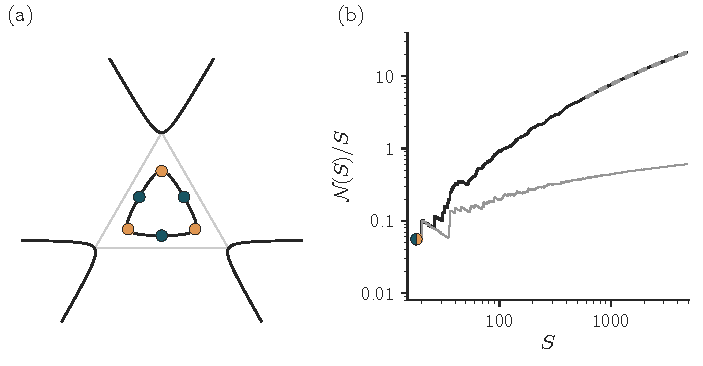
\includegraphics[width=119mm]{figures/out/F9.pdf}
\caption{(a) The real locus of $C_{27/2}$ in the chart $x+y+z=1$, with the permutations of $(1,4,4)$ (dark) and $(1,1,4)$ (orange). (b) The ratio $\N(S)/S$ for $S\le4800$ (heavy), a log-power fit (dashed), and the isosceles copies $k\mathcal D_{u,v}$ (thin).}\label{fig:F9}
\end{figure}

\subsection{What Question~\ref{q:intro} Would Require}\label{sec:heuristic}

By Theorem~\ref{thm:loglog} and Proposition~\ref{prop:upper}, the exponent of growth of $\N$ lies between $1$ and $3$. The local exponent is $1.58$ near $X=6000$ and still falling. The data are consistent with $\N(X)=X^{1+o(1)}$ and with $\N(X)$ growing like $X^{1.59}$; a finite range bounds the limiting exponent from neither side. The rest of this section is heuristic: we state what a positive answer to Question~\ref{q:intro} would say about the geometry.

\emph{Heuristic.} Parametric families are the natural source of many coincidences. Consider a family in which the entries of both triples are forms of degree $d$ in $m$ variables, with a generically finite parametrisation whose generic member is a pair of distinct triples. It contributes about $X^{m/d}$ pairs with sum at most $X$, up to logarithms and local densities. By Remark~\ref{rem:nolinear}, $d=1$ occurs, for forms in two variables, only through scaling. The isosceles family has $d=2$ and $m=2$: it is a rational \emph{curve} in the space of pairs up to scaling, and it gives $X\log X$ once the copies are counted. The dual family of Corollary~\ref{cor:dual} is a rational surface given by cubic forms in three variables ($d=3$, $m=3$); it is the quartic del Pezzo surface of Section~\ref{sec:lower}, and with their copies its pairs number $O(X(\log X)^5)$ and at least $X(\log X)^2$ in order of magnitude. A rational surface parametrised by quadratic forms in three variables ($d=2$, $m=3$) would give about $X^{3/2}$. Heuristically, then, a positive answer to Question~\ref{q:intro} would require that the variety of pairs contain no such surface whose positive real points form a nonempty open set. We have not searched for one: such a search ranges over surfaces in a threefold, not over lines in the plane, and we know no practical test. We searched for one-parameter families only: a line in $\PP^2$ of triples $(x:y:z)$ is a family linear in its parameter, and two lines (possibly equal) give a family of coincidences when $\Lambda$ agrees on them after a M\"obius change of parameter. We grouped the lines by the discriminant of the branch values of $\Lambda$ restricted to them and tested each candidate pair exactly. Among the $189$ lines $ax+by+cz=0$ meeting the positive triangle, with coprime integers $|a|,|b|,|c|\le7$, counted up to permutation of the coordinates and sign (the list and the test are in the deposit), the only such families are the conics of the dual family, one Vieta involution on each line through a vertex. Since $83.5\%$ of the primitive pairs up to $4800$ are neither dual nor of torsion type, the data do not show which subvarieties carry most of the coincidences.

The variety in question has a classical description. In coordinates, the pairs $(x,x')$ with $e_1(x)=e_1(x')$ and $e_2(x)e_3(x')=e_2(x')e_3(x)$ form a quintic hypersurface in the hyperplane $e_1(x)=e_1(x')$ of $\PP^5$. The map $(P,P')\mapsto(e_1(P')P,\,e_1(P)P')$ identifies pairs of points on a common $C_\Lambda$ with pairs of triples with equal sum and equal reciprocal sum. So the variety of pairs is birational to the fibre square $\mathcal E\times_{\PP^1}\mathcal E$ of the rational elliptic surface $\mathcal E\to\PP^1_\Lambda$ obtained by blowing up the base points of the pencil, nine counted with multiplicity. All singular fibres of $\mathcal E$ are of type $I_n$. Fibre products of rational elliptic surfaces were studied by Schoen \cite{schoen1988}, who obtained Calabi--Yau threefolds from them; we do not use this. The twelve surfaces $\{(P,\pm P+T)\}$, with $T$ in the group of base points, are graphs of automorphisms of the fibres; six of them consist of the orderings of $P$ itself, and the other six are the dual family in its six orderings, so Theorems~\ref{thm:iso} and~\ref{thm:loglog} both count points on one such surface. Over the curve of values $\Lambda=(r+1+1/r)^2$ the translations by the torsion points of order $12$ give further surfaces of this kind; their rational points lie over rational $r$, and for $r<0$ they carry the pairs of torsion type of Section~\ref{sec:growth}. Question~\ref{q:intro} concerns the positive rational points of this threefold off these surfaces as well, which come from positive-rank fibres over individual values of $\Lambda$.

\section*{Statements and Declarations}

\noindent\textit{Funding.} No funding was received for this work.

\noindent\textit{Competing interests.} The authors have no competing interests to declare that are relevant to the content of this article.

\noindent\textit{Data and code availability.} {\sloppy The code and data are at \url{https://github.com/pa1aash/equal-sum-reciprocal-triples}, archived at Zenodo \textbf{[PLACEHOLDER: Zenodo DOI]}, with all six authors as creators; the Zenodo record is the version to cite. One command reruns every check; the enumerations from scratch are rerun only on request. Table~\ref{tab:fibres} is produced by \texttt{make\_tables.py} from \texttt{groups.csv}, written by \texttt{enumerate\_fast.py}, and from the ranks of \texttt{ranks.py}; Table~\ref{tab:density} is produced by the same tool from \texttt{check\_enum.py} (to $S=6000$), cross-checked against \texttt{per\_S.csv}; the fits are those of \texttt{exponent\_fits.py} and \texttt{growth\_fits.py}, and Figure~\ref{fig:F9} is drawn by \texttt{F9.py}.\par}

\noindent\textit{Author contributions.} \textbf{[PLACEHOLDER: author contribution statement, to be supplied by the authors before submission.]}

\noindent\textit{Use of AI tools.} \textbf{[PLACEHOLDER: statement on the use of AI tools in preparing this manuscript, to be written by the authors.]}

\acknowledgements{The colours of Figure~\ref{fig:F9} are from the Scientific Colour Maps \cite{crameri2023}, which are designed to be perceptually uniform and readable by people with colour-vision deficiencies \cite{crameri2020}.}

\begin{thebibliography}{99}

\bibitem{beauville1982}
A. Beauville, Les familles stables de courbes elliptiques sur $\mathbf{P}^1$ admettant quatre fibres singuli\`eres, \textit{C. R. Acad. Sci., Paris, S\'er. I} \textbf{294} (1982), 657--660.

\bibitem{bremnerguy1997}
A. Bremner and R. K. Guy, Two more representation problems, \textit{Proc. Edinb. Math. Soc. (2)} \textbf{40}(1) (1997), 1--17.

\bibitem{bgn1993}
A. Bremner, R. K. Guy, and R. J. Nowakowski, Which integers are representable as the product of the sum of three integers with the sum of their reciprocals?, \textit{Math. Comp.} \textbf{61}(203) (1993), 117--130.

\bibitem{bremnermacleod2014}
A. Bremner and A. Macleod, An unusual cubic representation problem, \textit{Ann. Math. Inform.} \textbf{43} (2014), 29--41.

\bibitem{bremnermacleod2025}
A. Bremner and A. Macleod, Corrigendum: An unusual cubic representation problem, \textit{Ann. Math. Inform.} \textbf{62} (2025), 26--27.

\bibitem{bremnertho2018}
A. Bremner and Nguyen Xuan Tho, The equation $(w+x+y+z)(1/w+1/x+1/y+1/z)=n$, \textit{Int. J. Number Theory} \textbf{14}(5) (2018), 1229--1246.

\bibitem{browningelsholtz2011}
T. D. Browning and C. Elsholtz, The number of representations of rationals as a sum of unit fractions, \textit{Illinois J. Math.} \textbf{55}(2) (2011), 685--696.

\bibitem{browningsofos2019}
T. D. Browning and E. Sofos, Counting rational points on quartic del Pezzo surfaces with a rational conic, \textit{Math. Ann.} \textbf{373}(3--4) (2019), 977--1016.

\bibitem{cha2019}
B. Cha, A. Claman, J. Harrington, Z. Liu, B. Maldonado, A. Miller, A. Palma, T. W. H. Wong, and H. Yi, An investigation on partitions with equal products, \textit{Int. J. Number Theory} \textbf{15}(8) (2019), 1731--1744.

\bibitem{chen2025}
Chen Shuwen, A survey of the Prouhet--Tarry--Escott problem and its generalizations, preprint, arXiv:2506.11429, 2025.

\bibitem{choudhry2011}
A. Choudhry, Equal sums of like powers, both positive and negative, \textit{Rocky Mountain J. Math.} \textbf{41}(3) (2011), 737--763.

\bibitem{crameri2023}
F. Crameri, Scientific colour maps, version 8.0.1, Zenodo, 2023, \url{https://doi.org/10.5281/zenodo.8409685}.

\bibitem{crameri2020}
F. Crameri, G. E. Shephard, and P. J. Heron, The misuse of colour in science communication, \textit{Nature Communications} \textbf{11} (2020), 5444.

\bibitem{dggw2008}
E. B. Dryden, C. S. Gordon, S. J. Greenwald, and D. L. Webb, Asymptotic expansion of the heat kernel for orbifolds, \textit{Michigan Math. J.} \textbf{56}(1) (2008), 205--238.

\bibitem{dggw2017}
E. B. Dryden, C. S. Gordon, S. J. Greenwald, and D. L. Webb, Erratum to ``Asymptotic expansion of the heat kernel for orbifolds'', \textit{Michigan Math. J.} \textbf{66}(1) (2017), 221--222.

\bibitem{elsholtztao2013}
C. Elsholtz and T. Tao, Counting the number of solutions to the Erd\H{o}s--Straus equation on unit fractions, \textit{J. Aust. Math. Soc.} \textbf{94}(1) (2013), 50--105.

\bibitem{gangetal-heat}
P. Gang, A. Agadi, A. Veluri, J. Wang, J. Barreto, and A. Chouthaiwale, How much of a hyperbolic orbifold does heat hear?, preprint, \textbf{[PLACEHOLDER: preprint identifier]}.

\bibitem{graham1963}
R. L. Graham, A theorem on partitions, \textit{J. Austral. Math. Soc.} \textbf{3}(4) (1963), 435--441.

\bibitem{kelly1989}
J. B. Kelly, Partitions with equal products. II, \textit{Proc. Amer. Math. Soc.} \textbf{107}(4) (1989), 887--893.

\bibitem{kubert1976}
D. S. Kubert, Universal bounds on the torsion of elliptic curves, \textit{Proc. London Math. Soc. (3)} \textbf{33}(2) (1976), 193--237.

\bibitem{macleod2005}
A. J. MacLeod, Integer triangles with $R/r=N$, preprint, arXiv:math/0502475, 2005.

\bibitem{mazur1977}
B. Mazur, Modular curves and the Eisenstein ideal, \textit{Publ. Math. Inst. Hautes \'Etudes Sci.} \textbf{47} (1977), 33--186.

\bibitem{morelandzieve2013}
G. Moreland and M. E. Zieve, Some Diophantine equations related to positive-rank elliptic curves, preprint, arXiv:1304.1442, 2013.

\bibitem{tho2021}
Nguyen Xuan Tho, What positive integers $n$ can be presented in the form $n=(x+y+z)(1/x+1/y+1/z)$?, \textit{Ann. Math. Inform.} \textbf{54} (2021), 141--146.

\bibitem{pari2172}
The PARI Group, PARI/GP version 2.17.2, Univ. Bordeaux, 2025, \url{https://pari.math.u-bordeaux.fr/}.

\bibitem{sadekelsissi2015}
M. Sadek and N. El-Sissi, Partitions with equal products and elliptic curves, \textit{Osaka J. Math.} \textbf{52}(2) (2015), 515--525.

\bibitem{schinzel1996}
A. Schinzel, Triples of positive integers with the same sum and the same product, \textit{Serdica Math. J.} \textbf{22}(4) (1996), 587--588.

\bibitem{schoen1988}
C. Schoen, On fiber products of rational elliptic surfaces with section, \textit{Math. Z.} \textbf{197}(2) (1988), 177--199.

\bibitem{silvermantate2015}
J. H. Silverman and J. T. Tate, \textit{Rational Points on Elliptic Curves}, Undergraduate Texts in Mathematics, Springer International Publishing, 2015.

\bibitem{topyui2007}
J. Top and N. Yui, Explicit equations of some elliptic modular surfaces, \textit{Rocky Mountain J. Math.} \textbf{37}(2) (2007), 663--687.

\bibitem{ulas2013}
M. Ulas, A note on Diophantine systems involving three symmetric polynomials, \textit{J. Number Theory} \textbf{133}(10) (2013), 3283--3295.

\bibitem{vandoorn2025}
W. van Doorn, Partitions with prescribed sum of reciprocals: asymptotic bounds, preprint, arXiv:2502.02200, 2025.

\bibitem{ysv2024}
A. E. A. Youmbai, A. S. Zargar, and M. Voznyy, Partitions into triples with equal products and families of elliptic curves, \textit{Glas. Mat. Ser. III} \textbf{60}(1) (2025), 59--72.

\bibitem{zhang2016}
Y. Zhang, Integers representable as the product of the sum of four integers with the sum of their reciprocals, preprint, arXiv:1608.03382, 2016.

\bibitem{zhangcai2013}
Y. Zhang and T. Cai, $n$-tuples of positive integers with the same sum and the same product, \textit{Math. Comp.} \textbf{82}(281) (2013), 617--623.

\end{thebibliography}

\end{document}
